%*============================================================*
%**Goal		:   隔代同住对于青少年认知与非认知能力影响研究
%**Author	:  	 ZhangYi zhangyiceee@163.com 15592606739
%**Created	:  	 20200323
%**Last Modified: 2020
%*============================================================*



\documentclass{beamer}
\usepackage[UTF8,noindent]{ctexcap}
\usepackage{natbib}
\usepackage{hyperref}


\graphicspath{{figures/}}




\usetheme{Madrid}
%\usecolortheme{crane} %黄色
%\usecolortheme{wolverine} %黄蓝
%\usecolortheme{lily} %蓝白
%Information to be included in the title page:
\title[三代同住、隔代同住]{与祖辈同住对青少年认知与非认知能力影响研究}
\author{张毅}
\date{\today}

\begin{document}
\frame{\titlepage}
%开始你的边际贡献


\begin{frame}
\frametitle{摘要}
文章利用中国教育追踪调查2013-2014年数据研究了家庭居住结构对青少年认知与非认知能力的影响。研究结果表明,相较于核心家庭(父母双方均在家),扩展家庭(父母+祖辈)能显著提高青少年的认知与非认知能力,隔代家庭对于青少年的非认知能力有消极影响,但对其认知能力无显著影响。
\end{frame}

\begin{frame}
	\frametitle{背景}

	\begin{itemize}
	\item 青少年发展的重要性,人力资本理论
	\item 家庭在青少年发展中具有至关重要的作用
	\item 随着社会经济的发展,我国家庭居住结构也发生了变化,三代家庭以及隔代家庭的增加
	\end{itemize}
\end{frame}

\begin{frame}
	\frametitle{未归类的观点}
Children raised in two-biological-parent families tend to fare better academically than children raised in any other family form (Brown, 2010) 许多研究都表明在双亲家庭在学业上都比其他类型的居住模式好
\\ 家庭结构在是那个方面有影响(可以作为中间变量,来做机制检验)
\begin{itemize}
	\item 家庭经济条件:单亲家庭经济处于弱势
	\item 父母社会化:家长社会化解释的重点是育儿,首先是父母的教养实践。这里的论点是,与双亲家庭相比,单亲家庭、继父家庭和同居家庭中通常存在较弱的父母权威结构,监控和监督较少,这反过来又降低了儿童接受的养育质量
	\item 家庭不稳定:家庭结构的变化会造成负面影响,与家庭类型无关
\end{itemize}




\end{frame}


\begin{frame}
	\frametitle{Problem} 
%这一部分基本上是文献的梳理部分
	\begin{itemize}
		\item 与祖辈同住会不会对青少年产生影响?
		\item 国外相关文献较多
		\begin{itemize}
			\item 但国外居住成因与我国有差异
			\item 父母吸毒、犯罪等造成的与祖辈同住
 		\end{itemize}
		\item 国内相关研究刚起步,具有代表性的是吴愈晓的几篇研究\citep{吴愈晓2019,吴愈晓2018,张帆2020}
		\begin{itemize}
			\item 样本中存在的问题是低龄化,对于青少年相关研究关注不够
			\item 尽管国内学者也进行了探索,存在的问题是目前在定义上存在差异,如\citet{张帆2020}的定义中混有了隔代居住的样本,但本文认为隔代同住与三代同住之间仍存在结构性差异。
			\item 关注健康和认知能力较对,但是对于个体的非认知能力涉及不多(Heckman GED考试),认知与非认知能力对个体的未来收入有很好的预测作用,因此研究非认知能力非常重要
		\end{itemize}	
	\end{itemize}
\end{frame}


\begin{frame}
	\frametitle{Objective}
	本文的目标是研究与祖辈同住对于青少年发展的影响
	\begin{itemize}
		\item 描述三代同住、隔代同住和亲代同住之间在特征方面的差异;
		\item 研究与祖辈同住对青少年认知能力的影响;
		\item 研究与祖辈同住对青少年非认知能力的影响
	\end{itemize}
\end{frame}


\begin{frame}
	\frametitle{Approach}
数据来自中国教育追踪调查基线(2013-2014年)数据,运用多元线性回归并辅之以学校固定效应模型。
根据学生问卷中“这学期和你在家住的都有:”进行判断
	\begin{itemize}
		\item 亲代同住:与父亲和母亲同住
		\item 三代同住(拓展家庭):父亲+母亲+祖辈
		\item 隔代同住:只与祖辈同住
		\item 其他(不在本文研究范围内)
	\end{itemize}
	认知能力测量根据CEPS的调查直接使用;非认知能力借鉴前人研究进行借鉴,
\end{frame}

\begin{frame}
	\frametitle{Result1:与祖辈同住对于青少年认知能力的影响}
	\centering{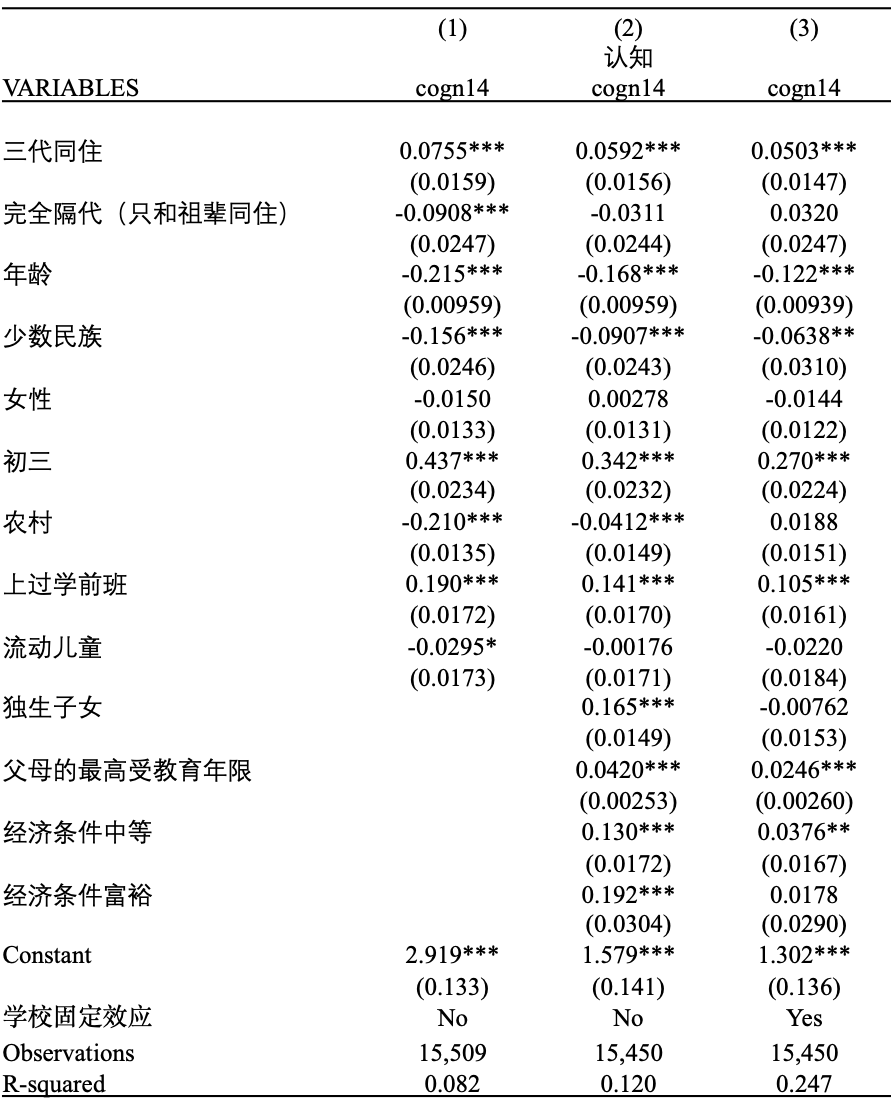
\includegraphics[scale=0.4]{table1}}
\end{frame}

\begin{frame}
	\frametitle{Result2:与祖辈同住对于青少年非认知能力的影响}
	\centering{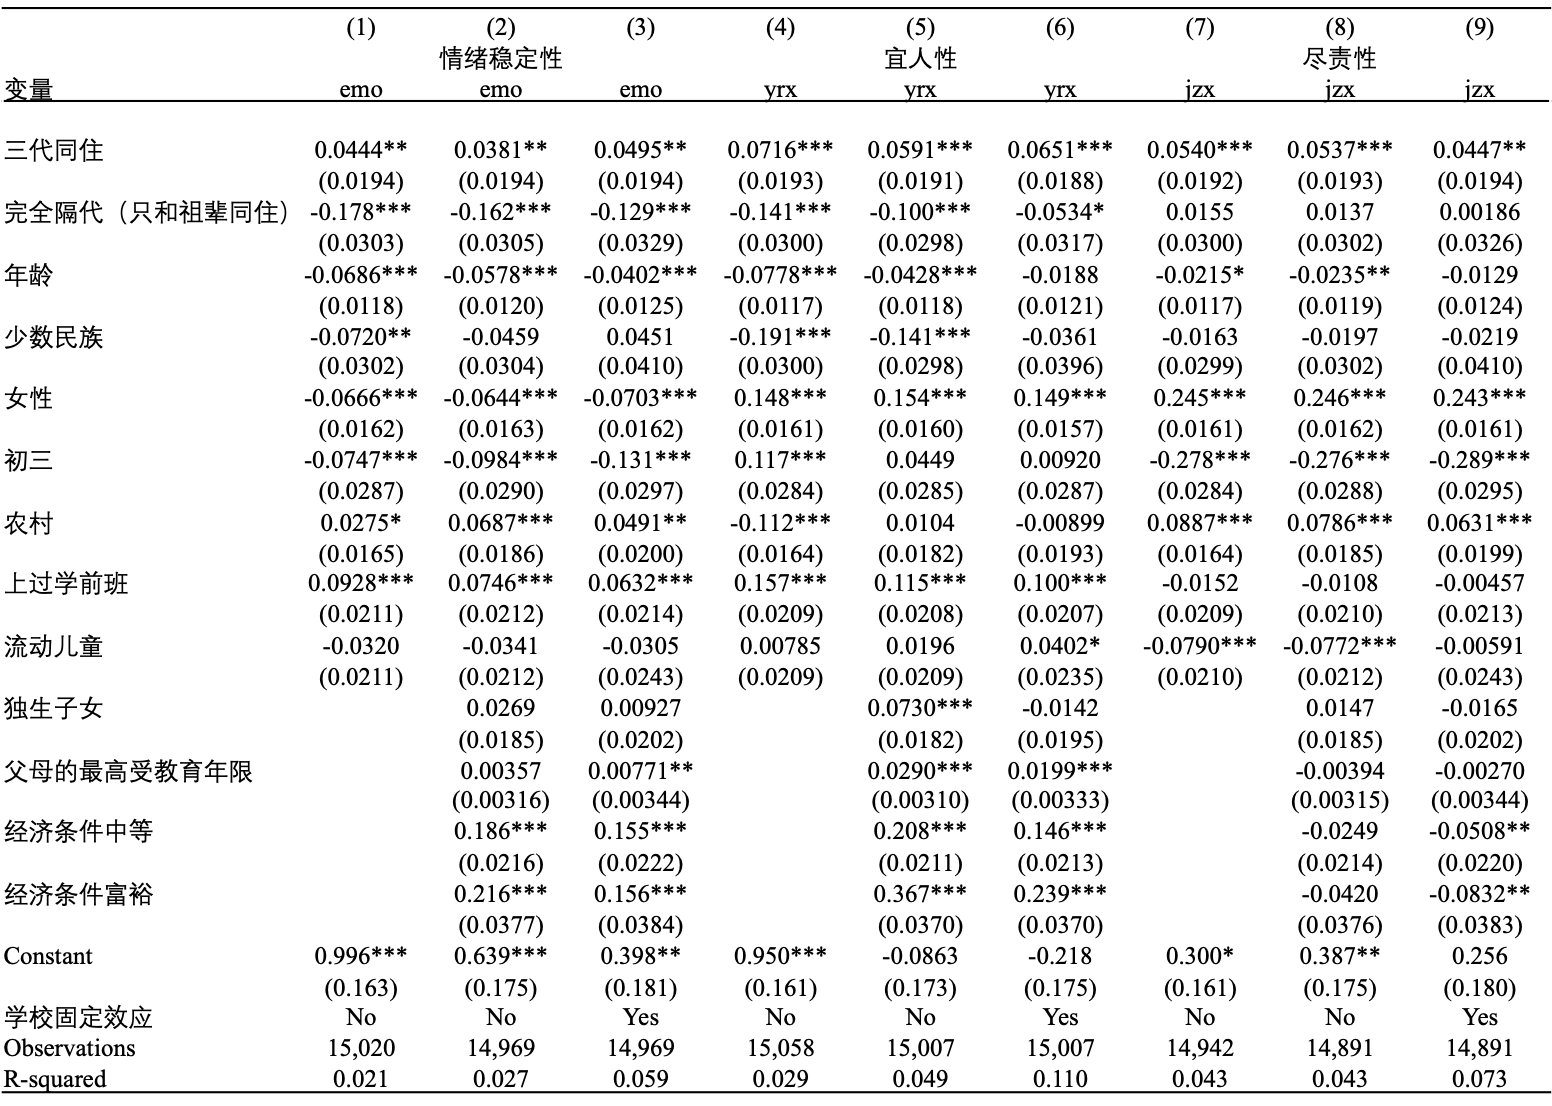
\includegraphics[scale=0.4]{table2}}
\end{frame}

\begin{frame}
	\frametitle{Discussion}
	可以看出三代同住对于青少年认知能力有显著的促进作用,隔代同住对于青少年认知能力没有显著影响
\\ 但从非认知能力来看,三代同住的家庭仍旧显示出对于青少年的正向影响,但是隔代同住对于青少年的情绪稳定性和宜人性有显著的负面影响。
\end{frame}

\begin{frame}
	\frametitle{局限}
	\begin{itemize}
		\item 数据的限制无法控制祖辈的相关信息
		\item 机制检验文中没有涉及,准备接下来进行补充

	\end{itemize}
\end{frame}


\begin{frame}
    \frametitle{参考文献}
\tiny
\bibliographystyle{plainnat}
\bibliography{references}
\end{frame}

%参考文献的案例 \citet{Krueger1999Experimental} \citep{Krueger1999Experimental}  注意两类的不同
\end{document}



